% !TEX root = PREN2_Dokumentation.tex
\section{Ideen und Konzepte}
\subsection{Vorwort}
Durch die \gls{PWA} \ac{JTI} Pick-Up Station ist es dem Kunden möglich, seine Ware bequem im Onlineshop zu bestellen und direkt und ohne Wartezeit an der gewünschten Pick-Up Station abzuholen. Durch den Prototyp sollen die Funktionalität und Zweckmässigkeit dieses für die Firma neuen Absatzkanals aufgezeigt werden. Im besten Fall findet die Applikation nicht nur in der Schweiz Verwendung, sondern wird von \ac{JTI} auch in anderen Märkten weltweit eingesetzt. Das Hauptaugenmerk der Arbeit liegt auf der Implementierung eines Prototyps mit den folgenden Schwerpunkten: Bestellung, Kauf, Nutzererfassung, Suche nach Pick-Up Stations und der Abholung an der Station. Bei der Nutzererfassung muss das Alter des Nutzers verifiziert werden. Die Lösung soll so weit als möglich in die Projektpartner-Systeme integriert werden. Hinzu kommt die Recherche von artverwandten Technologien und das Requirements Engineering. Die BDA wird als interdisziplinäre Bachelorarbeit durchgeführt. 

\subsection{Systemarchitektur}
Als Systemarchitektur stand die Erweiterbarkeit im Vordergrund. Allerdings sollte durch die Architektur die Applikation nicht unnötig komplex werden. Aus diesem Grund wurde bewusst gegen eine Microservicearchitektur entschieden. Die Umsetzung der Applikation mit Microservices würde zwar zu einer besseren Verteilbarkeit und Skalierung führen, der Aufwand und die Komplexität würde jedoch erheblich erhöht. \\
Es wurde auf eine Schichtenarchitektur gesetzt. Die klassische logische drei Schichtenarchitektur wurde noch weiter verfeinert, final wurde eine sechs Schichtenarchitektur entworfen. Die Architektur wird zusätzlich in 3 physische Tier aufgeteilt. 
\begin{figure}[H]
	\centering
	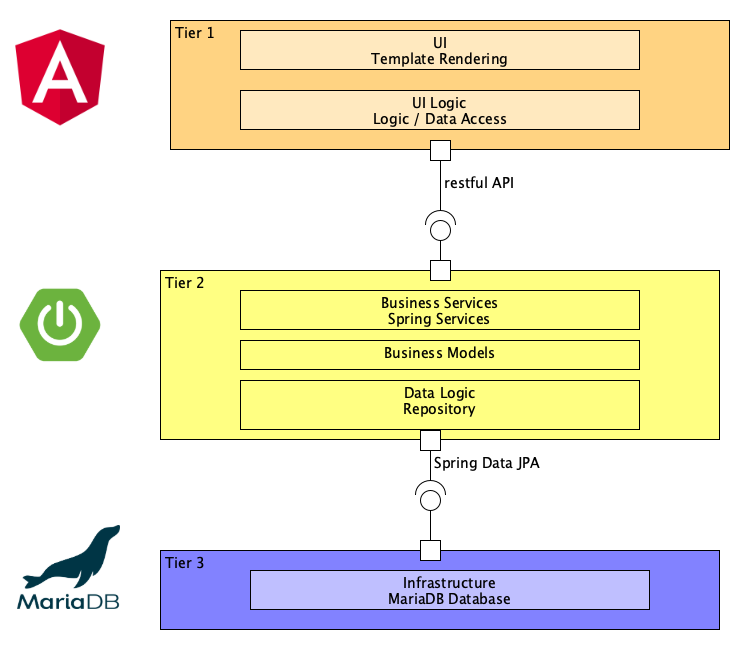
\includegraphics[scale=0.45]{images/architectureWithImages.png}
	\caption[Architektur]{Architektur, Quelle: Autor}
	\label{img: Architektur}
\end{figure}
\newpage
Die Architektur ermöglicht eine sehr gute Erweiterbarkeit. Zudem kann die Software verteilt werden und unabhängig voneinander skalieren. Durch die Aufteilung in sechs Tiers wird zudem vermieden, dass die einzelnen Tiers zu breit werden. Durch das Verwenden von Frameworks kann die Komplexität gering gehalten werden. Die Schnittstellen innerhalb der einzelnen Layer sind klar vorgegeben. Durch die Kommunikation via \ac{REST}, bzw. Repositories sind die Komponenten untereinander austauschbar. Die Kopplung ist sehr gering. 

\paragraph{UI}
Es wird eine Single-Page Applikation umgesetzt. Sie wird vorab im Browser geladen, später wird nur der entsprechende Inhalt neu aktualisiert. Das bringt eine verbesserte Nutzerexperience, da keine Abhängigkeiten zu Serverladezeiten bestehen. Hingegen dauert das initiale Laden länger [\cite{spa}]. 

\paragraph{UI Logic}
Aufgrund der gewählten Architektur werden die Daten der Applikation via \ac{REST}-Schnittstelle geladen. Das wird asynchron durchgeführt.

\paragraph{REST-Controller}
Die einzelnen \ac{REST}-Controller definieren die \ac{API}. Es wurden die folgenden Punkte bei der Erstellung berücksichtigt: 
  \begin{itemize}
	\item Konsistenz: Namensgebung und Regeln konsequent einhalten.
	\item Namensgebung: Einfache, eingängige, treffende Namen wählen.
	\item Verhalten: Klare Erwartungen erfüllen, ohne Nebeneffekte.
	\item Erweiterbarkeit: Offen für Weiterentwicklung (der API).
	\item Dokumentation: Einfache, hilfreiche, kompakte Dokumentation.
	\item Perspektive: Vom Anbieter für den Nutzer - es soll für den Nutzer einfach werden!
	\item KISS-Prinzip: Schnittstelle möglichst einfach halten.
	\item Sicherheit: Die Nutzung ist sicher zu gestalten.
\end{itemize}
[\cite{appeAPIDesign}]\\

Es wird gemäss Richardson Maturity Model \ref{img: richardsonMaturity} eine \ac{REST}-Schnittstelle von Level 3 angestrebt. 

\paragraph{Business Services}
Die Business Services kommunizieren mit den Domänenmodellen. Weitere Details werden im Abschnitt \ref{services} beschrieben. 

\paragraph{Business Models}
Es handelt sich um die Entities des Projekts. Sie werden aus dem Domänenmodell erarbeitet und sind einzigartig. Weitere Details werden im Abschnitt \ref{entity} beschrieben. 

\paragraph{Data Logic}
Zur Persistierung der Entities werden Repositories eingesetzt. Sie bilden die Schnittstelle zwischen Applikation und Datenbank. 
\newpage
\subsubsection{Zusammenspiel der einzelnen Layer}
\begin{figure}[H]
	\centering
	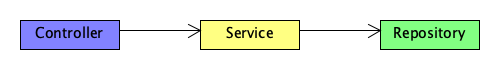
\includegraphics[width=\linewidth]{images/springFlow.png}
	\caption[Zusammenspiel von zentralen Layern]{Zusammenspiel von zentralen Layern, Quelle: Autor}
	\label{img: layer}
\end{figure}

\subsubsection{Infrastruktur}
Die gesamten Infrastruktur läuft im \gls{EnterpriseLab} der Hochschule Luzern. Das Front- und das Backend laufen auf unterschiedlichen virtuellen Maschinen. Die einzelnen Teilapplikationen sind als Docker-Container umgesetzt. 
\begin{figure}[H]
	\centering
	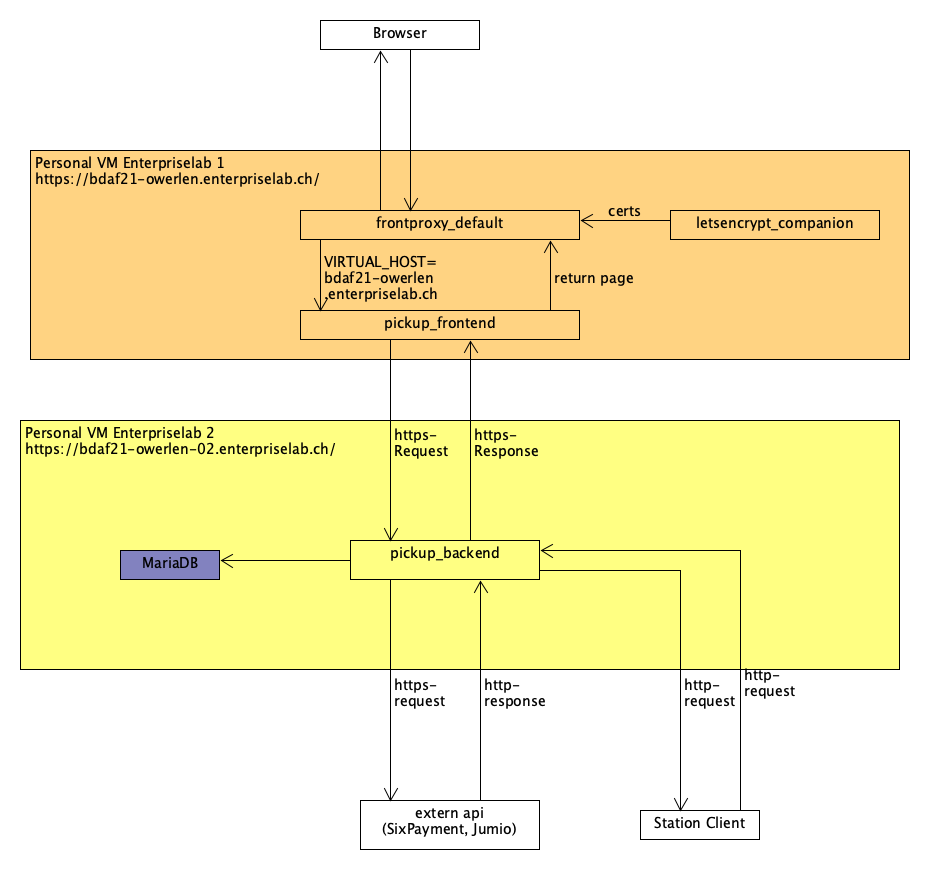
\includegraphics[width=\linewidth]{images/system.png}
	\caption[Container-Infrastruktur]{Container-Infrastruktur, Quelle: Autor}
	\label{img: Containerinfrastruktur}
\end{figure}
\newpage
Die beiden Diagramme \ref{img: Architektur} und \ref{img: Containerinfrastruktur} sind farblich identisch gehalten. 
Gesamthaft umfasst das System sechs Container.\\
Der Station-Client in diesem Diagramm befindet sich auf der physischen Station. Er ist das Bindeglied zwischen Informatik und Elektrotechnik und übernimmt Aufgaben wie die Produktausgabe oder das Inventar. 

\subsection{Mobile First}
Es werden erheblich mehr Websiteaufrufe von mobilen, als von Desktop Geräten registriert. Der mobile First Ansatz nimmt sich dieser Thematik an und besagt, dass die Applikation in einem ersten Schritt für mobile Geräte entwickelt wird. Der Fokus liegt auf dem Design der Seite, wohingegen die Performance ebenfalls berücksichtigt wird.\\
Die Bedeutung von mobile First hat durch Google dazugewonnen. Der mobile Index ist der primäre Index, die mobile Friendliness der ausschlaggebende Punkt beim Ranking von Suchergebnissen [\cite{mobileFirst}]. 
\subsection{Frameworks}
\subsubsection{\gls{Spring Boot}}
Spring Boot baut auf dem \gls{Spring} Framework auf. Es bietet sich an, um performante Enterprise-Applikationen mit Java zu erstellen. Spring Boot kann sehr einfach erweitert werden, sodass Spring Security, Spring MVC oder Spring Data eingesetzt werden können.\\
Spring Boot bringt einen integrierten Tomcat Server mit. Dies verringert den Konfigurationsaufwand. Es ist kein Einpacken in ein \gls{war} und zusätzliches deployen nötig. Zudem wird das Debugging erleichtert. Es übernimmt einen grossen Teil der Beans-Konfiguration von Spring [\cite{springBoot}].\\\\
Spring Boot bietet den grossen Vorteil, dass bereits Erfahrung in der Anwendung vorhanden ist. Es ist keine Einarbeitungszeit nötig, gängige Fehler können vermieden werden. Aus diesem Grund fiel die Entscheidung gegen Frameworks wie Node.js. 

\subsubsection{\gls{Angular}}\label{angularLabel}
Angular ist ein Application Design Framework, um effiziente Single Page Applikationen zu erstellen. Es basiert auf TypeScript [\cite{angular}]. Angular die Möglichkeit, als \gls{PWA} genutzt zu werden [\cite{angularPWA}]. 
Es wurde von Google entwickelt und bietet mit dem Material UI bereits viele Elemente, welche von nativen Android-Apps bekannt sind [\cite{angularMaterialUI}]. \\
Wie bei Spring ist in Angular bereits Projekterfahrung vorhanden. Ein Einarbeiten ist nicht mehr nötig, die gängigsten Funktionen sind bereits bekannt. \\
In vorhergehenden Projekten wurde das Frontend mit verschiedensten Technologien umgesetzt. Einerseits kam jQuery zum Einsatz, andererseits wurden auch Technologien wie \gls{React} genutzt. \gls{Angular} überzeugte von diesen Framework am meisten. Besonders durch die Unterstützung von \gls{TypeScript} fiel die Wahl auf dieses Framework. 
\newpage
\subsection{Weitere Technologien}
\subsubsection{Docker}
Docker ist eine Containertechnologie. Sie erlaubt die Erstellung und den Betrieb von Linux-Containern. Die Container sind dabei sehr leichtgewichtig und modular.\\
Die einzelnen Teile der Applikation werden in verschiedenen Containern betrieben [\cite{docker}].\\
Die Anwendung und Funktion von Docker wird in diversen Modulen an der Hochschule Luzern gelehrt. In vorhergegangenen Projekten wurde Docker bereits im selben Kontext genutzt. 

\subsubsection{MariaDB}\label{mariadb}
MariaDB ist ein OpenSource Datenbankmanagementsystem. Es ist durch die Abspaltung von MySQL entstanden und ein relationales Datenbanksystem. 
Aus Lizenzgründen wird in diesem Projekt MariaDB und nicht MySQL genutzt. Alternativ wäre auch ein Einsatz von PostgreSQL möglich. Der Unterschied zwischen PostgreSQL und MariaDB ist dabei nur marginal. Bei dieser Applikation wurde lediglich aus Erfahrung auf MariaDB gesetzt [\cite{mariadbVsPostgresql}]. \\
Durch die Verwendung von Spring Data wäre es möglich, die Datenbank im Verlauf des Projektes auszutauschen. 

\subsubsection{Hibernate ORM}
Hibernate ORM ist ein Object Relational Mapper. 
Er ermöglicht es dem Entwickler, einfacher mit der Datenpersistierung umzugehen. Hibernate ist zudem ein Teil der \ac{JPA} und der Spring Data JPA. 
Ein wichtiger Punkt ist die Performance, welche durch den Einsatz des Lazy Loading Patterns erreicht wird. Die Initialisierung des Objektes wird solange als möglich hinausgezögert. [\cite{hibernateORM}]

\subsubsection{\gls{GitLab}}
Zur Versionsverwaltung kam \gls{GitLab} zum Einsatz. Es wird dabei von der Hochschule Luzern zur Verfügung gestellt. Zudem sind zur Integration in die \gls{DevOps}-Umgebung bereits GitLab Runner vorhanden, um Docker Images zu erstellen. 

\subsubsection{Bezahldienst}
Als Bezahldienst wurde Saferpay von Six Payment Services genutzt. Dabei wurde mit der Testversion gearbeitet, diese unterscheidet sich nicht von der Produktiven. Ein Wechsel wäre zudem innert kurzer Zeit durchführbar. 

\subsubsection{Alterverifikation}
Bei der Altersüberprüfung wurde auf Jumio gesetzt. Das Produkt wurde vom Auftraggeber vorgegeben und eine Lizenz bereitgestellt. 

\subsubsection{Karte}
Für die Implementierung der Kartenfunktionalität wurde Leaflet genutzt. Die Kartendaten stammen von Open Street Map. Geoapify wurde als MapsAPI eingesetzt. 

\newpage